\documentclass{article}

\usepackage{amsmath, amssymb, float, xcolor, titlesec, tcolorbox}
\usepackage[hidelinks]{hyperref}
\usepackage{cleveref}
\usepackage{todonotes} % The notes can be hidden using \usepackage[disable]{todonotes}


% multireferenced footnotes
\makeatletter
\newcommand{\footnoteref}[1]{\protected@xdef\@thefnmark{\ref{#1}}\@footnotemark}
\makeatother


% Allow using pragraph as now subsubsubsection
\setcounter{secnumdepth}{4}
\titleformat{\paragraph}{\normalfont\normalsize}{\theparagraph}{1em}{}
\titlespacing*{\paragraph}{0pt}{3.25ex plus 1ex minus .2ex}{1.5ex plus .2ex}

% Box for stocks
\newtcolorbox{integ}{colback=white,grow to right by=-1mm,grow to left by=-1mm, boxrule=2pt,boxsep=0pt}

% Equation, figures, tables numbering
\newcommand{\prefix}[1]{
    \setcounter{equation}{0}
    \setcounter{figure}{0}
    \setcounter{table}{0}
    \renewcommand{\theequation}{#1.\arabic{equation}}
    \renewcommand{\thefigure}{#1.\arabic{figure}}
    \renewcommand{\thetable}{#1.\arabic{table}}
}

% Naming the models
\newcommand{\model}{\emph{pymedeas} }
\newcommand{\modelsub}[1]{\emph{pymedeas\_#1}}

% Commands for comments and other todos
\newcommand{\note}[1]{\todo[inline,color=orange]{{\bf TODO:} #1}}
\newcommand{\urgent}[1]{\todo[inline,color=red]{{\bf URGENT:} #1}}
\newcommand{\warning}[1]{\todo[inline,color=yellow]{{\bf WARNING:} #1}}
\newcommand{\eneko}[1]{\todo[inline,color=white,linecolor=red,bordercolor=red]{\textcolor{red}{\bf Eneko:} #1}}
\newcommand{\enric}[1]{\todo[inline,color=white,linecolor=green,bordercolor=green]{\textcolor{green}{\bf Enric:} #1}}
\newcommand{\roger}[1]{\todo[inline,color=white,linecolor=blue,bordercolor=blue]{\textcolor{blue}{\bf Roger:} #1}}
\newcommand{\jordi}[1]{\todo[inline,color=white,linecolor=yellow,bordercolor=yellow]{\textcolor{yellow}{\bf Jordi:} #1}}

% Titlepage
\title{\model models documentation}
\author{Eneko Martin-Martinez \and Enric Alcover \and Roger Samsó \and Jordi Solé}

\begin{document}
    \maketitle
    \note{use jcap to generate the authors}
    \note{include bibtex}
    \newpage
    \tableofcontents
    \newpage
    \listoftodos[TODOs]
    \newpage
    \section{General logic of the \model models}
        \label{se:general_logic}
        The MEDEAS models dynamically operate as follows: for each period, a sectoral economic demand is estimated from exogenous pathways of expected Gross Domestic Product per capita  (GDPpc) and population evolution. The final energy demand required to fulfil production is obtained using energy-economy hybrid input-output analysis, and energy intensities by type of final energy. The energy sub-module computes the available final energy supply, which may or may not satisfy demand, adapting the economic production to the available energy. The materials required by the economy, with emphasis on those required by alternative green technologies, are estimated; this allows to assess eventual future mineral bottlenecks. The new energy infrastructure requires energy investments, whose computation allows to estimate the variation of the EROI (Energy Return over Energy Invested) of the system, which in turn affects the final energy demand. The climate submodule computes the greenhouse gas (GHG) emissions associated to the resulting energy mix (complemented by exogenous pathways for non-energy emissions), which feeds back to the economy, affecting final demand. Additional land requirements are accounted for. Finally, the social and environmental impacts are computed. For more detail the reader is referred to Refs. --> **all this is taken from [@SAMSO2020100582] and needs to be either cited or modified**


\urgent{Update the general logic of pymedeas}



    \section{Main hypothesis behind the \model models}
        \label{se:hypothesis}
        \urgent{Write main hyphothesis}
Lorem ipsum dolor sit amet, consectetur adipiscing elit. Sed hendrerit, lacus nec vehicula viverra, nibh leo lacinia erat, ullamcorper sodales leo elit nec metus. Duis leo erat, vulputate eget ultricies ac, fringilla at nibh. Nam fringilla nec nibh nec scelerisque. Morbi fermentum dui in lectus placerat, at porta augue blandit. Fusce sagittis quam a elit ultricies, at euismod velit interdum. Pellentesque nibh massa, auctor vitae commodo at, ultrices in nunc. Phasellus sapien arcu, venenatis vel est accumsan, interdum aliquam enim.

Mauris ut dignissim lacus, tristique congue nibh. Proin volutpat eros et nisl pharetra condimentum. Suspendisse sagittis lacus tellus, id fermentum quam suscipit in. Integer aliquet gravida tellus, sed varius nulla facilisis ac. In tortor enim, aliquet vitae purus non, hendrerit aliquet ante. Proin et iaculis erat. Ut eu mattis urna, eget iaculis lorem. Vivamus euismod ligula nec vestibulum consequat. Aenean quis tortor quis ipsum sollicitudin fringilla in vel justo. Phasellus lectus ex, rutrum ac ultrices id, ullamcorper vitae metus. Morbi nec velit velit. Donec varius posuere neque, sed pellentesque dui efficitur vitae. Suspendisse sed quam scelerisque risus fermentum sagittis vitae ut leo.

Donec eleifend facilisis efficitur. Sed suscipit tortor tellus, placerat sodales velit faucibus sed. Suspendisse porta, leo a venenatis suscipit, elit nulla interdum tellus, sed ultricies purus arcu sit amet sapien. Aenean dolor nisi, convallis vitae condimentum ac, consectetur a magna. Proin non feugiat purus. Sed pharetra, mi vel egestas varius, orci velit bibendum sem, ut porta diam sapien id ante. Phasellus posuere dignissim magna, nec sollicitudin ex fringilla sed. Donec dictum id orci ac consectetur. Nam fringilla orci malesuada ipsum maximus, luctus tempor diam suscipit.

Aenean sed erat fermentum, ullamcorper elit sit amet, semper ante. Sed suscipit vitae est sed rhoncus. Vestibulum in posuere turpis. Suspendisse finibus ex velit, non condimentum sapien viverra sit amet. Praesent eu sapien nec massa convallis suscipit ac ac nunc. Nunc ut ullamcorper est. Vestibulum a urna quis urna finibus suscipit quis sed velit. Nulla aliquam tincidunt nisl quis tempus. Duis nec ex a mauris imperdiet fermentum non tempor ligula. Curabitur sed nibh quis nisi tincidunt tincidunt quis a purus. Maecenas sit amet nisl vel lacus pharetra tincidunt. Donec placerat arcu sollicitudin tempus faucibus. Integer et turpis egestas, fermentum massa lobortis, dignissim mi. Sed semper urna fermentum tellus dignissim auctor.

In facilisis porta tortor. In eleifend sed enim at laoreet. Suspendisse vitae gravida magna. In dictum sapien tempor orci iaculis, nec efficitur nisl tristique. Vivamus molestie vestibulum leo, iaculis pulvinar lacus interdum egestas. Curabitur rhoncus arcu non ligula dapibus, a pulvinar dolor vulputate. Vivamus tristique, orci eu dapibus blandit, nisl lectus pharetra orci, ut sodales sem velit egestas lacus. 

\citep{SAMSO2020100582}

    \section{Main features of the \model models}
        \label{se:features}
        \subsection{Nestings}
            \label{se:nestings}
            The \model models allow to run from whole world experiments to small scale regions. In order to do so, three pymedeas models are provided, which are organized in two nestings:
\begin{itemize}
    \item The main model is the full world model (nesting level 0). This model repressents the full agreggated world system. This model is also called \modelsub{w}.
    \item The first nested model (nesting level 1) corresponds to a regional model, this model repressents a region of the world model. This model is also called \modelsub{rg}.
    \item The second nested model (nesting level 2) corresponds to a subregional model, this model repressents a subregion of the region used in the regional model.  This model is also called \modelsub{srg}.
\end{itemize}

\begin{figure}[H]
    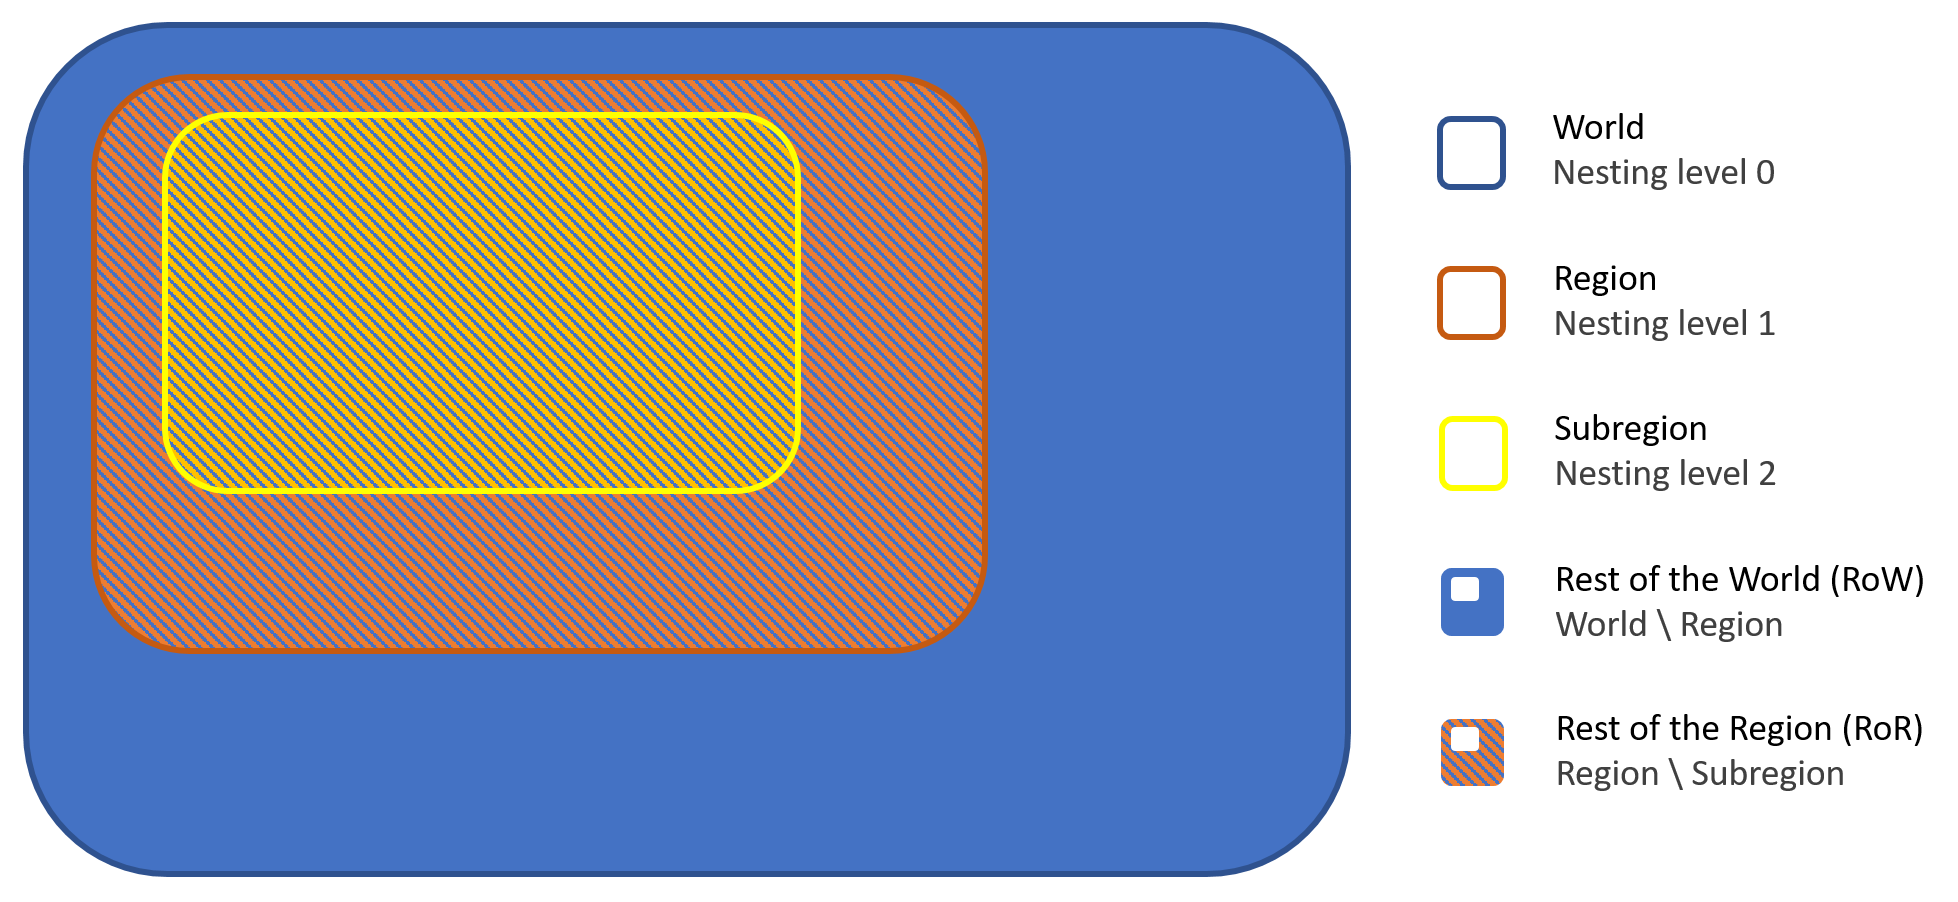
\includegraphics[width=\textwidth]{figures/nesting.png}
    \caption{Nesting of \model models}
    \label{fig:nesting}
\end{figure}

In the nested models we commonly refer to the complementary part of the region as rest of the world (RoW) or rest of the region (RoR). Therefore, Row repressents all the world except Region, and RoR repressents all the Region except Subregion, see the Figure \ref{fig:nesting}.

In order to run a nested model the upper... \note{Add runing nested models information}


    \section{Modules}
        \label{se:modules}
        \subsection{Climate}
            \label{se:climate}
            \prefix{CLIM}
            \subsubsection{Estimation of GHG emissions}

The model computes the $CO_2$ and $CH_4$ emissions associated to the extraction and burning of fossil fuels. While $CO_2$ emissions are produced during the combustion of fossil fuels, $CH_4$ emissions are originated by the losses of methane during extraction, processing, tranmission and distribution, notably of natural gas. Biofuels are far from being neutral carbon emitters due to Indirect Land Use Changes (ILUC); hence, in accordance with (\enric{cites}), we assign a similar emission level than natural gas. Emissions factors are considered constant over time. 

The module has incorporated the capability of calculating the emissions by each economic sector and final source. In such a way, it can be determined which of the sectors is the most polluting in terms of GHG and, from here, be able to design transition scenarios in which the activity of these sectors can be reduced. 

When one form of primary energy is transformed into another type of energy,for example burning gas to generate electricity, these emissions must be linked to the consumption of the final source (electricity) and not to that of the primary energy (gas). The same goes for heat generation and liquid transformation technologies (GTL, CTL). At the same time, when we have a cogeneration plant (CHP) that generates electricity and heat, we must distribute the fuel emissions that have been generated between the electricity consumer and the heat consumer. In this case, the share of electricity and heat is calculated as:

\begin{equation}
    Sh\_Elect\_CHP_i= \frac{Elec\_CHP_i}{Elec\_CHP_i+Heat\_CHP_i}
    \label{eq:share-elec-CHP}
\end{equation}


Where $Sh\_Elect\_CHP_i$ is the share of primary energy $i$ (gas, oil or coal), $Elec\_CHP_i$ is the potential electricity generation from CHP plants burning primary energy, and $Heat\_CHP_i$ is the final energy demand of $i$ in CHP plants. 

Then, the share of each of the primary energies for heat and electricity is obtained from:

\begin{equation}
    Sh\_Elect_i= \frac{PE\_Elect_i+PED\_CHP_i \cdot Sh\_Elect\_CHP_i}{PED_i}
    \label{eq:share-elect-i}
\end{equation}


\enric{General description of the module}

\paragraph{}
        \subsection{Economy}
            \label{se:economyy}
            \prefix{ECON}
            \note{Document real demand computation process (economy evolution)}
\note{Include final energy intensities in this section}


\note{Create a template to introduce all module inputs in the same way}
Module inputs:
\begin{itemize}
    \item Capital compensation per sector
    \item Labour compensation per sector
    \item Gross fixed capital formation per sector
    \item Household demand per sector
    \item Goverment expenditures per sector
    \item Change in inventories per sector
    \item Final demand by sector of other regions per sector\footnote{\label{fnote:regional-var}This variables are only required in the nested models, and are the export from the running region to the rest of the parent regions.}
    \item Export of final goods to other regions per sector\footnoteref{fnote:regional-var}
    \item Final energy intensities per sector and final source
    \item Gross Domestic Product (GDP)
    \item Economic coefficient A matrix for the wanted sectors\footnote{Coefficient matrix should be given in the dessagregation of the current level, if the input is for a subregion, the first submatrix should be for the subregion the second for the rest of the region and the last for the rest of the world.}
\end{itemize}

Scenario parameters:
\begin{itemize}
    \item GDPpc growth
    \item LC and CC growth policies...
\end{itemize}
\note{Add information about the module and scenario inputs}

\subsubsection{Final demand}
    \label{se:economy-final_demand}
    The final demand ($FD$) is the basis of the economic evolution of pymdedeas models. For the computation of the final demand the expected Gross Domestic Product ($GDP$) evolution is used.

\paragraph{Capital and labour compensations}

\warning{
    This process is split in different submodules:
        pymedeas\_w: sectors\_and\_households
        pymedeas\_eu: gdp\_desired\_labour\_and\_capital\_share
        pymedeas\_cat: gdp\_desired\_labour\_and\_capital\_share
}

Capital compensation ($CC$) and labour compensation ($LC$) are used in the models to compute the time evolution of final demands. This values are computed from a share of the gross domestic product ($GDP$).

Both capital and labour compensations are computed in a similar ways. First the expected $GDP$ of next step (time $i\!+\!1$) is computed, using the expected growth ($GDPgrowth^{i}_{expc}$), which is  given as an scenario input by the user. This process is given in equation \eqref{eq:exp_gdp}.

\begin{equation}
GDP_{expc}^{i+1} = GDP^i\,(1+GDPgrowth^{i}_{expc})
\label{eq:exp_gdp}
\end{equation}

The expected capital compensation share ($CCshare$) and labour compensations share ($LCshare$) respect to the $GDP$ are computed following their expected growth as given in equations \eqref{eq:exp_ccshare} and \eqref{eq:exp_lcshare}, respectively.

\begin{gather}
CCshare_{expc}^{i+1} = CCshare^i\,(1+CCgrowth_{expc}) \label{eq:exp_ccshare}\\
LCshare_{expc}^{i+1} = LCshare^i\,(1+LCgrowth_{expc}) \label{eq:exp_lcshare}
\end{gather}

Therefore, the expected $CC$ and $LC$ are computed in equations \eqref{eq:exp_cc} and \eqref{eq:exp_lc} using the product of expected $GDP$ and their corresponent expected share.

\begin{gather}
CC_{expc}^{i+1} = GDP_{expc}^{i+1} \, CCshare_{expc}^{i+1}\label{eq:exp_cc}\\
LC_{expc}^{i+1} = GDP_{expc}^{i+1} \, LCshare_{expc}^{i+1}\label{eq:exp_lc}
\end{gather}

Therefore, when putting together equations \eqref{eq:exp_gdp} to \eqref{eq:exp_lc} the expected variation of $LC$ and $CC$ can be computed as follows given in \eqref{eq:exp_cc2} and \eqref{eq:exp_lc2}.

\begin{gather}
\Delta CC_{expc}^i = GDP^i\,CCshare^i\,\Big[\left(1+GDPgrowth^{i}_{expc}\right)\,\left(1+CCgrowth_{expc}\right)-1\Big]\label{eq:exp_cc2}\\
\Delta LC_{expc}^i = GDP^i\,LCshare^i\,\Big[\left(1+GDPgrowth^{i}_{expc}\right)\,\left(1+LCgrowth_{expc}\right)-1\Big]\label{eq:exp_lc2}
\end{gather}

Finally, the new step $LC$ and $CC$ are corrected using the total uncovered demand ($UD_{total}$) of the current step as shown in equations \eqref{eq:cc_next} and \eqref{eq:lc_next},

%\begin{integ}
    \begin{equation}
    CC^{i+1} = CC^i+\Delta CC_{expc}^i-UD_{total}^i\,CCshare_{expc}^i\label{eq:cc_next}
    \end{equation}
%\end{integ}
%\begin{integ}
    \begin{equation}
    LC^{i+1} = LC^i+\Delta LC_{expc}^i-UD_{total}^i\,LCshare_{expc}^i\label{eq:lc_next}
    \end{equation}
%\end{integ}

\warning{Current version of pymedeas\_cat doesn't take into account the uncovered demand to compute the CC and LC!}
\warning{In the world model the CC is computed by sectors CC(sector), maybe we should compute the total directly in order to have the same approach in the 3 models.}

\paragraph{Gross fixed capital formation and households demand}
\label{par:gfcf_hd}
\warning{
    This process is split in different submodules:
        pymedeas\_w: sectors\_and\_households
        pymedeas\_eu: households\_economic\_demand / exports\_demand
        pymedeas\_cat: households\_economic\_demand\_and\_investment
}

The gross fixed capital formation ($GFCF$) and households demand ($HD$) by sector at time $i$ are computed asuming the relations of equations \eqref{eq:loggfcf} and \eqref{eq:loghd}, respectively.

\begin{gather}
\log\left(GFCF^i(sector)\right) = b_0^{GFCF}(sector) + b_1^{GFCF}\,\log\left(CC^i\right)\label{eq:loggfcf}\\
\log\left(HD^i(sector)\right) = b_0^{HD}(sector) + b_1^{HD}\,\log\left(LC^i\right)\label{eq:loghd}
\end{gather}

where $b_x^y$ parameters are adjusted by doing a linear regression with historical data. Being $CC$ and $LC$ the capital and labour compensations respectively.

From the equations \eqref{eq:loggfcf} and \eqref{eq:loghd} the new relations from \eqref{eq:vargfcf} and \eqref{eq:varhd} to compute the expected variation in $CC$ and $LC$.
\begin{gather}
\Delta GFCF^i_{expc}(sector) = e^{b_0^{GFCF}(sector)}\,\Big[\left(CC^i\!+\!\Delta CC_{expc}^i\right)^{b_1^{GFCF}}-\left(CC^{i}\right)^{b_1^{GFCF}}\Big]\label{eq:vargfcf}\\
\Delta HD^i_{expc}(sector) = e^{b_0^{HD}(sector)}\,\Big[\left(LC^i\!+\!\Delta LC_{expc}^i\right)^{b_1^{HD}}-\left(LC^{i}\right)^{b_1^{HD}}\Big]\label{eq:varhd}
\end{gather}


Finally the new step $GFCF$ and $HD$ are corrected using the uncovered demand by sector ($UD$) of the current step, see equations \eqref{eq:gfcf_next} and \eqref{eq:hd_next}.
%\begin{integ}
    \begin{align}
    GFCF^{i+1}(sector) =\hspace{5pt}  &GFCF^i(sector)+\Delta GFCF^i_{expc}(sector)\nonumber\\
                        &-UD^i(sector)\,GFCFshare^i_{expc}(sector)\label{eq:gfcf_next}
    \end{align}
%\end{integ}
%\begin{integ}
    \begin{align}
    HD^{i+1}(sector) =\hspace{5pt}  &HD^i(sector)+\Delta HD^i_{expc}(sector)\nonumber\\
                    &-UD^i(sector)\,HDshare^i_{expc}(sector)\label{eq:hd_next}
    \end{align}
%\end{integ}

\warning{In the world model the CC is used by sectors.}

\paragraph{Exports demand}
The exports demand is only computed in nested models. In the case of the regional model, the exports to the \emph{rest of the world} (RoW) are needed, while, in the case of the subregional model the exports to the \emph{rest of the region} (RoR) and \emph{rest of the world} (RoW) are needed.

The computation of the exports demand ($ExpD$) is similar to that used for gross fixed capital formation and households demand in Section
\ref{par:gfcf_hd}.
\begin{equation}
\log\left(ExpD^i_{ExpRoX}(sector)\right) = b_0^{ExpRoX}(sector) + b_1^{ExpRoX}\,\log\left(GDP^i_X\right)\label{eq:logexp}
\end{equation}

The equation \eqref{eq:logexp} shows the logarithmic relation of the exports to rest of region $X$ (RoX) based on the gross domestic product of $X$ ($GDP_X$), where $X$ could be \emph{world} or \emph{region}. The parameters $b_x^y$ are adjusted by doing a linear regression with historical data. Therefore, the expected variation is computed as given in equation \eqref{eq:varexp}.
\begin{align}
\Delta ExpD^i_{RoX,\,expc}(sector) =\hspace{50pt}& \nonumber\\e^{b_0^{ExpRoX}(sector)}&\,\Big[\left(GDP^{i+1}_X\right)^{b_1^{ExpRoX}}-\left(GDP^i_X\right)^{b_1^{ExpRoX}}\Big]\label{eq:varexp}
\end{align}

Finally the new step $GFCF$ and $HD$ are corrected using the uncovered demand by sector ($UD$) of the current step, equation \eqref{eq:exp_next} show how the stock of $ExpD$ is computed.
%\begin{integ}
    \begin{align}
    ExpD^{i+1}_{RoX}(sector) = \hspace{5pt}&ExpD^i_{RoX}(sector)+\Delta ExpD^i_{RoX,\,expc}(sector)\nonumber\\
    &-UD^i(sector)\,ExpD_{RoX}share^i_{expc}(sector)\label{eq:exp_next}
    \end{align}
%\end{integ}


\paragraph{Change in inventories and goverment expenditures}

\warning{
    This process is split in different submodules:
        pymedeas\_w: sectors\_and\_households
        pymedeas\_eu: economic\_demand
        pymedeas\_cat: economic\_demand
}

The share of change in inventoris and goverment expenditures ($CI\&GEshare$) respect to the final demand is assumed constant after the historic period. This way the goverment expenditures and change in inventories contribution to the finall demand ($CI\&GE$) by sector at time $i$ is computed using the values for gross fixed capital formation ($GFCF$), household demand ($HD$) and exports demand ($ExpD$) by sector, as given in equation \eqref{eq:cigeshare}.
\begin{align}
CI\&GE^i(sector)=\frac{CI\&GEshare}{1-CI\&GEshare}\,\Big[&GFCF^i(sector)+HD^i(sector)\nonumber \\&+ExpD^i(sector)\Big]\label{eq:cigeshare}
\end{align}


\paragraph{Final demand}

\warning{
This process is split in different submodules:
        pymedeas\_w: sectors\_and\_households
        pymedeas\_eu: economic\_demand
        pymedeas\_cat: economic\_demand
}

The final demand $FD$ is the sum of gross fixed capital formation ($GFCF$), households demand ($HD$), change in inventories and goverment expenditures ($CI\&GE$) and exports demand ($ExpD$). Therefore, the $FD$ by sector at time $i$ can be computed as given in equation \eqref{eq:fd1}.
\begin{align}
FD^i(sector) =\hspace{5pt} &GFCF^i(sector)+HD^i(sector)\nonumber\\
               &+ExpD^i(sector)+CI\&GE^i(sector)\label{eq:fd1}
\end{align}

When combining equation \eqref{eq:fd1} with \eqref{eq:cigeshare} the $FD$ can be given as in equation \eqref{eq:fd2}.
\begin{equation}
FD^i(sector)=\frac{GFCF^i(sector)+HD^i(sector)+ExpD^i(sector)}{1-CI\&GEshare}
\label{eq:fd2}
\end{equation}

Therefore, the expected change in the final demand is computed using the expected change of all the variables from equation \eqref{eq:fd2}. The output of resulting equation \eqref{eq:varfd} is used together with the uncovered demand in order to compute the final demand in the next step in equation \eqref{eq:fd_next}.

\begin{align}
\Delta FD_{expc}^i&(sector)=\nonumber\\
&\frac{\Delta GFCF_{expc}^i(sector)+\Delta HD_{expc}^i(sector)+\Delta ExpD_{expc}^i(sector)}{1-CI\&GEshare}
\label{eq:varfd}
\end{align}

%\begin{integ}
    \begin{equation}
    FD^{i+1}(sector)=FD^i(sector)+\Delta FD_{expc}^i(sector)-UD^i(sector)
    \label{eq:fd_next}
    \end{equation}
%\end{integ}

 \subsubsection{Total outputs}
    \label{se:economy-total_outputs}
    \paragraph{Energy intensities}
\note{include information about energy intensities}

\paragraph{Coefficient matrices}
\note{include information about coefficient matrices}

\paragraph{Total outputs from demand}
\note{include information about total outputs}


        \subsection{Energy}
            \label{se:energy}
            \prefix{ENER}
            This module is in charge of the estimation of energy demand, the energy supply, the energy resource availability, the modelling of electricity and heat generation and the modelling of non-energy use. The module is diveded in 6 submodules:

\begin{itemize}
    \item Availability
    \item Demand
    \item EROI
    \item Storage
    \item Supply
\end{itemize}

\eneko{Please Enric, add cross-reference in the equations use a standard for adding the label (e.g. $\backslash$label\{eq:oil-demand\})}
\subsubsection{Availability}
    \label{se:energy-availability}
    \note{Oil extraction, reformulate in only one way}
\note{Gas extraction, reformulate in only one way}
\note{Explain year scarcity}
\note{Explain nuclear}


The availability of non-renewable energy sources is calculated by each of the sources included in the model: oil, natural gas, coal and uranium.
The model considers the following non-renewable energy resources:

\begin{enumerate}
    \item Conventional oil: refers to crude oil and NGLs.
    \item Unconventional oil: includes heavy and extra-heavy oil, natural bitumen (oil sand and tar
    sands) and oil shales. Biofuels, CTL, GTL and refinery gains are modeled separately.
    \item Conventional gas.
    \item Unconventional gas: includes shale gas, tight gas, coal-bed methane (CBM) and hydrates.
    \item Coal: includes anthracite, bituminous, sub-bituminous, black, brown and lignite coal.
    \item Uranium
\end{enumerate}

Nuclear fusion is not considered since the ITER and DEMO projects
estimate that the first commercial fusion power would not be available before 2040, which would prevent this technology to substantially contribute to the mix
in the timeline of MEDEAS.

The availability of non-renewable energy resources in MEDEAS depends upon two constraints:

\begin{enumerate}
    \item Stock: available resource in the ground
    \item Flow: extraction rate of this resource
\end{enumerate}

The available stock of a resource is usually measured in terms of ultimately recoverable resources
($URR$), or remaining RURR ($RURR$) if referenced to a given year. The RURR in a given time t is defined
as the difference between the URR and cumulative extraction ($CExt$) in time t:

In order to estimate the future availability of fossil fuels, we have reviewed the studies providing
depletion curves for non-renewable energy resources taking into account both stocks and flow
limits. 

The depletion curves of non-renewable energies reviewed in the literature represent extraction
levels compatible with geological constraints as a function of time. As the model is demand based, we assume that, while the maximum extraction rate is not reached, the extraxction of each resource matches the demand. Actual
extraction will therefore be the minimum between the demand and the maximum extraction rate. To do this, the depletion curves have been converted into maximum production
curves as a function of remaining resources. In these curves, as long as the remaining resources are
large, extraction is only constrained by the maximum extraction level. However, with cumulated
extraction, there is a level of remaining resources when physical limits start to appear and maximum
extraction rates are gradually reduced. In this way, the model uses a stock of resources (the RURR)
and it studies how this stock is exhausted depending on production, which is in turn determined by
demand and maximum extraction.

\begin{equation}
    RURR_t=URR - CExt_t
    \label{eq:available_stock}
\end{equation}
    
\enric{Add  Literature review of depletion curves by fuel}

\paragraph{Oil Extraction}
The limitation of the oil resources, and availability of oil depends on two constraints: the stock (EJ) and the flows (Watts). The model priorizes the others NRE liquids fuels, then the oil demand is obtained as follows:

\begin{equation}
Oil_{demand}=PED_{NRE\_Liquids}-FES_{CTL}- FES_{GTL}- ORF
\label{eq:oil-demand}
\end{equation}

Where $PED\_NRE\_Liquids$ is the Primary energy demand of non-renewable eneregy liquids (EJ), $FES\_GTL$ is the final energy demand of GTL (Gas-to-liquids) (EJ),  FES\_CTL is the final energy demand of GTL (Coal-to-liquids) (EJ) and ORF is the oil refinery gains.

\paragraph{Natural gas extraction}

\paragraph{Coal extraction}

Coal extraction submodule is in charge of obtaining the coal extraction taking into account the limitations of the coal resources. The model priorizes other solid NRE sources for satisfying the primary energy demand.

\begin{equation}
Coal_{demand}=PED_{solids}-PE_{trad\_bio}-PES_{peat}-PES_{waste}-LCP
\label{eq:coal-demand}
\end{equation}

Where, $PED\_solids$ is the primary energy demand of the solids (EJ), $PE\_trad\_bio$ is the primary energy of the traditional biomass (EJ), $PES\_peat$ is the Primary energy suplly of peat (EJ), PES\_waste is the primary energy obtained from waste (EJ) and LCP are the losses in charcoal plants (EJ).

The amount of coal that can be extracted is limited by the Hubbert curves if the parameters *unlimited coal?* and *unlimited NRE?* are desactivated. Then, the extraction of coal is limited by the maximum extraction limit as:

\begin{equation}
Coal_{extraction}=min(PED_{coal}, max\_extract\_coal))
\label{eq:coal-extraction}
\end{equation}

\paragraph{Uranium extraction}

Uranium extraction depends on demand and resource availability, taking into account the Hubbert curve of maxim extraction of the uranium. The demand of uranium is obtained from the potential generation of nuclear electricity divided by the efficiency of uranium for electricity. If the parameters *unlimited uranium?* and *unlimited NRE?* are desactivated, the extraction of uranium is limited by the maximum extraction limit as:
\eneko{Avoid talking about parameters like unlimited uranium or unlimited NRE, they are used for research but their non-default value has no physical sense!}

\begin{equation}
Uranium_{extraction}=min(PED_{uranium}, max\_extract\_uranium))
\label{eq:uranium-extraction}
\end{equation}

In the nested models, for calculating the abundance of uranium, the imports from the rest of the world are included. In such way, when there is local scarcity, the imports can compensate it.

\warning{There can be a double counting of imports of the RoW of the nested model of Europe and the nested model of Catalonia!}

\paragraph{Final energy abundance}

The abundance of final fuels is obtained from the primary energy demand (PED) and the primary energy supply (PES) as follows:

\begin{equation}
A= \frac{PED_i-PES_i}{PED_i}
\label{eq:abundance-final-fuels}
\end{equation}

When the $PED<PES$ the abundance is always 1. The index i is the energy carrier: liquids, gases, solids, electricity and heat.
Then, depending on the \emph{sensitivity to scarcity option} defined in the scenarios files, the perception of final energy scarcity of each fuel by economic sectors is obtained. This perception drives the fuel replacement and efficiency improvement. This perception of scarcity decreases on time depending on the \emph{energy scarcity forgeting time} defined also at the scenario files as the time in years that society takes to forget the percepticon of scarcity for economic sectors.

\paragraph{Renewable energy sources (RES) availability}

Although renewable energy is usually considered a huge abundant source of energy, there are technological and ecological limits to its development. . However, the large scale deployment of renewable alternatives faces serious challenges in relation to their integration in the electricity mix due to their intermittency, seasonality and uneven spatial distribution requiring storage, their lower energy density, their dependence on minerals and materials for the construction of power plants and related infrastructures and their associated environmental impacts, that pose problems on its fast and global growth. All this factors significantly reduce their sustainable potential.
 
\enric{Include bibliography (A lot of information at the deliverable 4.1)}

\enric{Detail all RES availability}


\subsubsection{Demand}
    \label{se:energy-demand}
    \note{Describe demand submodule}

\subsubsection{EROI}
    \label{se:energy-eroi}
    \note{Describe EROI submodule}

\subsubsection{Storage}
    \label{se:energy-storage}
    \note{Describe storage submodule}

\subsubsection{Supply}
    \label{se:energy-supply}
    Primary total energy demand is covered with different Primary Energy Sources (PES) gruped in five categories: solids, liquids, gases, electricity and heat



% \begin{table}
%     \textbf{MEDEAS final energy category} ; \textbf{NRE / RES} ; \textbf{Energy source modelled in MEDEAS}
% \end{table}
    

\paragraph{Nuclear}

Installation of nuclear plants is limited by several factors: uranium availability, RES supply, nuclear Cp.

There are four different scenarios
\begin{enumerate}
    \item Constant power at current levels
    \item No more nuclear power installed capacity
    \item Growth of nuclear power installed capacity
    \item Phase-out nuclear power
\end{enumerate}

In the firts one, the nuclear capacity is being substitute when the lifetime of the installations is reached; in the second scenario, there is not more nuclear power installed when the facilities are depreciated; in the third scenario there is a yearly increase of the power capacity; and in the phase-out scenario there is a decrease of nuclear facilities before its lifetime is reached.

The new annual increase of new planned nuclear capacity is zero except for the scenario 3, where this increase of capacity is defined in the scenario's excel. Then, the new requiered capacity is obtained by:

\begin{equation}
C_{new \_nuc}=   C_{nuc} \cdot G_{nuc\_elect} \cdot Ef_{scarcity\_uranium} \cdot Cp_{limit}
\label{eq:new-nuc-capacity}
\end{equation}

Where $C\_num$ is the actual installed capacity, $G\_nuc\_elect$ is the annual growth of new planned nuclear capacity, $Ef_{scarcity\_uranium}$ is the efect of uranium scarcity and Cp limit is a factor that limitates the new capacity installation when the capacity factor of nuclear due to the RES penetration falls below 60\%.

The efects of the uranium scarcity, that is calculated in the availabilty submodule, con be modeled by a relationship that avoids an abrupt limitation by introducing a range (1;0.8) in the uranium abundance that constrains the development of new nuclear facilities. This relation models the behaviour of new required nuclear capacity when the abundance is in the range (1;0.8):

\begin{equation}
Ef_{scarcity\_uranium}=  ((A_{Uranium}-0.8) \cdot 5)^2
\label{eq:effects-uranium-scarcity}
\end{equation}

Then, the new planed nuclear capacity is calculated from the new nuclear capacity under planning plus replacement nuclear capacity less nuclear capacity under construction.

\paragraph{Solar potentials in urban areas}


\paragraph{RES electricity potentials}

Nine types of RES for electricity generation are modeled: hydro, solar PV, solar CSP, onshore wind, offshore wind, geothermal, biomass, oceanic and biogas.

Renewables potentials are limited by biophysical sustainable constraints, limiting the potential installed by a techno-sustainable limits that are taking into account the ecological, and the technical limitation of renewable energy sources. This potential limits are read from the "energy.xslx" excel file.

\paragraph{RES electric capacities and generation}

Renewable Energy Source (RES) capacity from different sources (hydro, geothermal, solid biomass, oceanic, wind onshore, wind offshore and solar) is limited by the techno-ecological potentials and its growth is defined in the "scenario.xslx" file, with objectives policies of total capacity installed by each RES every 5 years.  
Then, this desired capacity is limited by the techno-ecological potential, that is defined at "energy.xlsx" file and with values obtained from literature. 

Energy output of the installed capacity is afected by two main sources: the capacity factor and curtailment. Capacity factor (Cp) variation has been discussed in literature, some sources, as \cite{IEA2022}, proposed increasing values of Cp as RES penetration level increases. Others, as \cite{NREL2012}, proposed a decreasing Cp proportional to the renewable share in the electricity generation mix. In our model, a constant Cp obtained from historical data is used. 

The other limiting factor is curtailment. Increased variable RES penetration levels may drive a system to encounter transmission or operational constraints, forcing the system operator to accept less wind or solar than is available, in this cases, curtailment takes part of the electricity generated. As this factor depends on several parameters \cite{Bird2016} as  infrastructural, operational, or institutional development of the grid, as well as the development of an storage technology that can manage the peak generation electricity, it depends on several policies and strategies. This parameter is defined at the scerario's file as a share of total potential renewable electricity generated. 
 
The module prioritize the use of biogas and waste as energy sources, and only after consuming this energy, other RES sources are taked into account.

\enric{Revisar}


\paragraph{RES electric supply by technology}

There is a priority in RES, first of all, electricity generation from waste and bioenergy is calculated and the final electricity demand after priorities obtained as:

\begin{equation}
    FED_{elect\_after\_prior}= FED_{elect\_tot}-FES_{elect\_bio}-FES_{elect\_waste}
    \label{eq:FED-after-priorities}
\end{equation}

Then, $FED_{elect\_after\_prior}$ is used by the RES electricity potential submodule for determining the amount of RES potential to be installed.
Once the model has calculated the total amount of electricity generated from RES, it obtains the electricity demand from NRE that is needed to satisfy the total electricity demand as:

\begin{equation}
    FED_{elect\_NRE}= FED_{elect\_tot}-FES_{RES}-FES_{elect\_waste}
    \label{eq:FED-elect-NRE}
\end{equation}


\paragraph{RES electric overcapacity due to RES variability}

The most abundant RES for the generation of electricity, solar and wind, are subject to temporal variability. Variable RES are characterized by short-term (e.g., cloudiness. day-night) and seasonal variability. A renewable mix scenario allows to partially mitigate the variablity of different RES. However, this complementarity is far from the compensation of different sources. In any region there is a certain probability of extreme combinations in the availability of natural resources. Moreover, there can be large annual variations in the availability of natural resources; for instance, the output of wind turbines in any given area can vary by up to 30\% from one year to the next.  It has been estimated that current electricity systems and grids can usually accommodate up to only 20\% electricity from renewable sources without a need for dedicated storage facilities. Thus, a certain level of: (1) storage, (2) grid development (3) overcapacity and/or (4) flexible demand management should then be considered if a high penetration RES electricity system is designed.


Overcapacities are limited by the economic profitability of the power plant (i.e. large overcapacities imply low Cp). From a net energy perspective, overcapacities tend to lower the EROI, which could  similarly affect the net energy profitability of the plant.

The RES for electricity generation can be classified as “baseload”, i.e. those sources that are able to supply a manageable (“dispachtable”) load such as hydro, 13 biomass and geothermal, and “variable” generation. The latter are characterized by differing levels of variability and limited predictability over various time scales, and include wind and solar technologies.

Overcapacity of RES energy generation is obtained from:

\begin{equation}
    Oc= PS_{RES}/FES_{RES}
    \label{eq:Overcapacity}
\end{equation}

Where $PS_{RES}$ is the Potential supply of RES sources and $FES_{RES}$ is the real final energy supply obtained.

\paragraph{RES electric total monetary investment}

The monetary investment for building new plants up to 2050 is computed following (Teske et al.,
2011). We assume the same price to new plants and repowering plants, in order to not understimate the cost. 

The costs related to the variability of RES and the need of grid development are modeled taking into account studies for wind. Grid reinforcement costs are obtained from the median value calculated in (Mills et al., 2012)  for 40 transmission studies for wind energy
in the USA.

Other monetary costs, as balancing costs, are also introduced into the model. We assume here similar costs for the combined variable
renewable producers -solar and wind-, extrapolating the cost until it reaches a maximum of 8
euros/MWh (7.6 US 1995\$/MWh) at 50\% of total electricity share.

\enric{Detail monetary investments}

\paragraph{Electricity generation from CHP plants}

The development of these plants is estimated as a function of the remaining commercial heat demand that is not covered by renewables sources. Tendencies are maintained. Once commercial heat produced in CHP plants is estimated to cover the demand, CHP plants efficiencies are used to obtain the electricity produced
in each of these plants.


        \subsection{Environment}
            \label{se:environment}
            \prefix{ENV}
            \note{Document environment module}
\subsubsection{Land}
    \label{se:environment-land}
    \note{Document land submodule}

    \subsubsection{Water}
    \label{se:environment-water}
    \note{Document water submodule}

        \subsection{Materials}
            \label{se:materials}
            \prefix{MAT}
            \note{Document materials module}
        \subsection{Society}
            \label{se:society}
            \prefix{SCTY}
            \paragraph{Population}

This view calculates the evolution of the population from exogenous drivers. There are three different ways to obtain the population evolution: From SSPs, from timeseries introduced manually or from annual constant variation. In this way, the population growth follows an independent evolution from other variables.

\warning{The population submodule has to be revised introducing some limitation on the population growth, that can depend on the GDP, the damage function, etc.}

\paragraph{Social and environmental impacts}

This view relates the biophysicals results with social and environmental indexes. There is a need of indetifying factors that influence social welfare by covering more aspects than only income levels. Thios social welfare indicators are influenced byeconomic variables such as population and GDP, but also connected to climate module.

The first calculated index is the Human Development Index. It has been observed that above certain level of GDP, the HDI decouples from income. Therefore it is important to consider other relations that may explain the HDI evolution. Among these, energy consumption is found to have an importnat relation, so it is used by the model, following the next equation:

\begin{equation}
    HDI=0.1508+0.1395 \cdot ln(TFEC_{pc})
\end{equation}

\warning{The correlation of the HDI with the TFEC is not the best approax, it can be approximated by the relation with the Final Energy Footprint per capita (FEFpc) (Deliverable 4.1)}

Then the carbon footprint per capita and the water use per capita are calculated dividing the total ammounts by the population. Finally, the CO2 emissions per value added is obtained dividing the total CO2 emissions by the GDP.
        \subsection{Transport}
            \label{se:transport}
            \prefix{TRANS}
            \note{Document transport module}


\end{document}
